\documentclass{article}%
\usepackage[T1]{fontenc}%
\usepackage[utf8]{inputenc}%
\usepackage{lmodern}%
\usepackage{textcomp}%
\usepackage{lastpage}%
%
\usepackage{amsmath}%
\usepackage{amssymb}%
\usepackage{amsfonts}%
\usepackage{graphicx}%
\usepackage{hyperref}%
\usepackage{tikz}%
\usepackage{pgfplots}%
\usetikzlibrary{math}%
\title{ITA 2026 - Física\thanks{This exam was solved and automatically generated with gpt-resolve: \url{https://github.com/lgabs/gpt-resolve}}}%
\author{claude{-}opus{-}5{-}5 (solver) + claude{-}opus{-}5{-}5 (judge)}%
\date{November 10, 2026}%
%
\begin{document}%
\normalsize%
\maketitle%
\section*{Questão 1}

\section*{Solução}

\textbf{Modelo.} Como $R$ é muito maior que as dimensões do trem, todas as rodas descrevem praticamente o mesmo raio. Por isso o trem pode ser tratado como partícula (não são dados a altura do centro de massa nem a bitola, então não há equação de torque a usar). Com velocidade constante, a única aceleração é a centrípeta, $a_c=v^2/R$, horizontal e apontando para o centro da curva. Não há força longitudinal: velocidade constante e resistências desprezadas. Assim, o atrito de cada roda atua no plano transversal, ao longo da geratriz do cone.

\textbf{Geometria do contato.} Pela figura, cada roda tem raio maior do lado interno, junto ao eixo. Logo, no ponto de apoio a superfície cônica faz ângulo $\theta$ com a horizontal, e a normal que o trilho exerce sobre a roda faz ângulo $\theta$ com a vertical, inclinada para o centro do trem. Na roda externa à curva (índice 1), essa normal aponta para o centro da curva. Na roda interna (índice 2), ela aponta para fora da curva. Somam-se as forças de todas as rodas de um mesmo lado.

Seja $\tan\varphi=\mu$. Como $|f_i|\le \mu N_i$, a força total de contato $\vec F_i=\vec N_i+\vec f_i$ forma com a normal um ângulo de no máximo $\varphi$ (cone de atrito). Medindo ângulos a partir da vertical, positivos para o centro da curva:
\[
\alpha_1\in[\theta-\varphi,\;\theta+\varphi],\qquad \alpha_2\in[-\theta-\varphi,\;-\theta+\varphi].
\]

\textbf{a)} Segunda lei de Newton, com $X_i$ e $Y_i$ as componentes horizontal (centrípeta) e vertical de $\vec F_i$:
\[
X_1+X_2=\frac{Mv^2}{R},\qquad Y_1+Y_2=Mg .
\]
Suponha $\theta+\varphi<90^\circ$. Então todos os $\alpha_i$ estão em $(-90^\circ,90^\circ)$, logo $Y_i\ge 0$, e
\[
X_i=Y_i\tan\alpha_i\le Y_i\tan(\theta+\varphi).
\]
Somando as duas rodas:
\[
\frac{Mv^2}{R}\le Mg\tan(\theta+\varphi).
\]
A igualdade exige que toda a força venha da roda externa, no limite de escorregamento ($f_1=\mu N_1$, dirigido para baixo e para o centro, contra a tendência da roda de "subir" no trilho). Isso significa $N_2=0$: a roda interna está na iminência de perder o contato. Para $R$ menor, não existe distribuição de forças com $N_2\ge 0$ e o trem descarrila. Portanto
\[
R_{\min}=\frac{v^2}{g\tan(\theta+\varphi)}=\frac{v^2\,(1-\mu\tan\theta)}{g\,(\tan\theta+\mu)}=\frac{v^2(\cos\theta-\mu\sin\theta)}{g(\sin\theta+\mu\cos\theta)} .
\]
Isso vale para $\mu\tan\theta<1$. Se $\mu\tan\theta\ge 1$ (ou seja, $\theta+\varphi\ge 90^\circ$), nesse modelo nenhum raio faz as rodas perderem o contato e não há mínimo positivo.

Conferência pelo limiar $N_2=0$: as equações $N_1\sin\theta+\mu N_1\cos\theta=Mv^2/R$ e $N_1\cos\theta-\mu N_1\sin\theta=Mg$ dão a mesma razão $v^2/(Rg)=\tan(\theta+\varphi)$.

\textbf{b)} Sem atrito ($\mu=0$), cada força é puramente normal:
\[
(N_1+N_2)\cos\theta=Mg,\qquad (N_1-N_2)\sin\theta=\frac{Mv^2}{R}.
\]
Então
\[
N_2=\frac{M}{2}\left(\frac{g}{\cos\theta}-\frac{v^2}{R\sin\theta}\right)\ge 0
\;\Longrightarrow\;
R_{\min}=\frac{v^2}{g\tan\theta},
\]
que coincide com o item (a) para $\mu=0$. É o mesmo resultado de uma curva sem atrito com inclinação $\theta$.

\textbf{c)} Rodas cilíndricas ($\theta=0$): as normais são verticais, com $N_1+N_2=Mg$, e só o atrito lateral fornece a força centrípeta:
\[
\frac{Mv^2}{R}=f_1+f_2\le \mu(N_1+N_2)=\mu Mg
\;\Longrightarrow\;
R_{\min}=\frac{v^2}{\mu g}.
\]
Para $R$ menor, as rodas escorregam lateralmente para fora dos trilhos. O resultado coincide com o item (a) para $\theta=0$.

\textbf{Verificações.} Todas as respostas têm a forma $v^2/g$, que tem dimensão de comprimento (m). Como $\tan(\theta+\varphi)>\tan\varphi$ e $\tan(\theta+\varphi)>\tan\theta$, o raio mínimo de (a) é menor que os de (b) e (c). Isso confirma que a conicidade das rodas melhora a aderência em curvas.

\medskip
ANSWER: a) $R_{\min}=\dfrac{v^2(1-\mu\tan\theta)}{g(\tan\theta+\mu)}$ (para $\mu\tan\theta<1$; se $\mu\tan\theta\ge1$, não há mínimo); b) $R_{\min}=\dfrac{v^2}{g\tan\theta}$; c) $R_{\min}=\dfrac{v^2}{\mu g}$.%
\newpage%
\section*{Questão 2}

\section*{Solução}

\textbf{Hipóteses e referencial.} Usamos o eixo $x$ ao longo do plano, apontando para cima da rampa, com origem na extremidade inferior da barra, e o eixo $y$ perpendicular ao plano. Com isso, as posições ficam:
\[
x_A=d,\qquad x_B=L-d,\qquad x_M=\tfrac{L}{2}\ \text{(barra homogênea)},\qquad x_m=a,\qquad x_{C}=L-b .
\]
Cada peso $Pg$ se decompõe em $Pg\cos\theta$, perpendicular ao plano (no sentido do plano), e $Pg\sin\theta$, paralela ao plano (rampa abaixo). Em cada apoio atuam a normal $N_i$ (perpendicular ao plano) e o atrito estático $f_i$ (ao longo do plano). Supomos desprezíveis a espessura da barra e a altura dos apoios, já que o enunciado não fornece essas medidas. Assim, as componentes paralelas ao plano têm linha de ação sobre o eixo da barra e não geram torque em relação a A ou a B. Para a barra em repouso, valem $\sum\vec F=\vec 0$ e $\sum\tau=0$ em relação a qualquer ponto.

\subsection*{a) Forças normais}

Tomando torques em relação a $A$, a força $N_A$ e os dois atritos não contribuem. Sobra:
\[
N_B\,(L-2d)=g\cos\theta\left[M\left(\tfrac{L}{2}-d\right)+m\,(a-d)+m_C\,(L-b-d)\right].
\]
Tomando torques em relação a $B$:
\[
N_A\,(L-2d)=g\cos\theta\left[M\left(\tfrac{L}{2}-d\right)+m\,(L-a-d)+m_C\,(b-d)\right].
\]
Daí:
\[
\boxed{N_A=g\cos\theta\left[\frac{M}{2}+\frac{m\,(L-a-d)+m_C\,(b-d)}{L-2d}\right]},\qquad
\boxed{N_B=g\cos\theta\left[\frac{M}{2}+\frac{m\,(a-d)+m_C\,(L-b-d)}{L-2d}\right]}.
\]
Pela 3ª lei de Newton, as forças trocadas entre apoio e plano têm esses módulos e são perpendiculares ao plano.

\emph{Verificação.} Somando as duas expressões, $N_A+N_B=(M+m+m_C)\,g\cos\theta$, que é o equilíbrio na direção $y$. As unidades estão corretas: kg$\cdot$m/s$^2$ = N. Se $m=m_C=0$, obtemos $N_A=N_B=\tfrac{Mg\cos\theta}{2}$, como exige a simetria. Se $a=d$, o peso de $m$ vai inteiramente para $A$. Para que a barra não tombe, é preciso $N_A\ge 0$ e $N_B\ge 0$. Essa é a função do contrapeso quando $m$ fica fora do vão entre os apoios. Na configuração da figura ($d<a<L-d$, $d<b<L-d$), as duas normais são positivas.

\subsection*{b) Forças de atrito}

O equilíbrio na direção $x$ dá:
\[
f_A+f_B=(M+m+m_C)\,g\sin\theta ,
\]
com os dois atritos apontando rampa acima. Os torques não fornecem nova equação, pois os atritos e as componentes paralelas dos pesos têm a mesma linha de ação. Portanto, a estática da barra rígida determina apenas a soma dos atritos.

Para obter cada atrito, supomos que os dois apoios são do mesmo material, com coeficiente $\mu$. Como a barra é rígida, ela só desliza se os dois apoios deslizarem juntos. O deslizamento é impedido se existirem $f_A\le\mu N_A$ e $f_B\le\mu N_B$ com a soma acima, ou seja, se
\[
(M+m+m_C)\,g\sin\theta\le\mu\,(N_A+N_B)=\mu\,(M+m+m_C)\,g\cos\theta\iff\mu\ge\tan\theta .
\]
O coeficiente mínimo que impede o deslizamento é então $\mu_{\min}=\tan\theta$. Nessa situação de deslizamento iminente, a soma $f_A+f_B$ é igual a $\mu(N_A+N_B)$, e cada parcela vale no máximo $\mu N_i$. Logo, cada parcela atinge o seu máximo: $f_A=N_A\tan\theta$ e $f_B=N_B\tan\theta$. Assim:
\[
\boxed{f_A=g\sin\theta\left[\frac{M}{2}+\frac{m\,(L-a-d)+m_C\,(b-d)}{L-2d}\right]},\qquad
\boxed{f_B=g\sin\theta\left[\frac{M}{2}+\frac{m\,(a-d)+m_C\,(L-b-d)}{L-2d}\right]},
\]
ambos paralelos ao plano e apontando rampa acima.

\emph{Verificação.} A soma dá $f_A+f_B=(M+m+m_C)\,g\sin\theta$. Para $\theta=0$, os atritos se anulam, como esperado num plano horizontal. Para $m=m_C=0$, cada apoio recebe $\tfrac{Mg\sin\theta}{2}$. Os atritos são proporcionais às normais, na razão $f_i/N_i=\tan\theta$.

\medskip
ANSWER: a) $N_A=g\cos\theta\left[\frac{M}{2}+\frac{m(L-a-d)+m_C(b-d)}{L-2d}\right]$ e $N_B=g\cos\theta\left[\frac{M}{2}+\frac{m(a-d)+m_C(L-b-d)}{L-2d}\right]$, com $N_A+N_B=(M+m+m_C)g\cos\theta$. b) $f_A=N_A\tan\theta=g\sin\theta\left[\frac{M}{2}+\frac{m(L-a-d)+m_C(b-d)}{L-2d}\right]$ e $f_B=N_B\tan\theta=g\sin\theta\left[\frac{M}{2}+\frac{m(a-d)+m_C(L-b-d)}{L-2d}\right]$, rampa acima. A soma $f_A+f_B=(M+m+m_C)g\sin\theta$ é sempre determinada; a divisão entre os apoios supõe o mesmo $\mu$ nos dois e $\mu_{\min}=\tan\theta$.%
\newpage%
\section*{Questão 3}

\section*{Solução}

\textbf{Hipóteses e geometria.} A haste é rígida e homogênea, e o pivô é ideal (sem atrito), de modo que sobre ela agem só o peso $M\vec g$, aplicado no centro de massa (CM), e a reação $\vec R$ do pivô. O CM está no ponto médio da haste. Pela figura, $a<L/2$, então o CM fica no trecho longo, a uma distância
\[
d=\frac{L}{2}-a=\frac{L-2a}{2}
\]
do pivô. Seja $\hat r$ o versor que aponta do pivô para o CM, ao longo da haste. Com os eixos da figura, $\hat r=(\sin\theta,\,-\cos\theta)$.

\textbf{Cinemática do CM.} O CM descreve uma circunferência de raio $d$ centrada no pivô. Sua aceleração tem:
\begin{itemize}
\item uma componente centrípeta $\omega^2 d$, dirigida para o pivô (sentido $-\hat r$);
\item uma componente tangencial $\alpha d$, perpendicular a $\hat r$.
\end{itemize}
A aceleração angular $\alpha$ não aparece na direção radial. Por isso a componente radial da reação não depende de $\alpha$.

\textbf{a)} Pelo teorema do movimento do centro de massa, $\vec R+M\vec g=M\vec a_{CM}$. Projetamos essa equação em $\hat r$. Como $\vec g=(0,-g)$, temos $\vec g\cdot\hat r=g\cos\theta$, e então
\[
R_r+Mg\cos\theta=-M\omega^2 d
\quad\Longrightarrow\quad
R_r=-M\left[\omega^2\,\frac{L-2a}{2}+g\cos\theta\right].
\]
O sinal negativo indica que, para $\theta<90^\circ$, a componente radial aponta do CM para o pivô, ou seja, ao longo da haste e para o centro de rotação. Seu valor é
\[
\boxed{F_r=M\left[\frac{\omega^2(L-2a)}{2}+g\cos\theta\right]}
\]
em módulo e orientada para o pivô. Em forma vetorial, $\vec F_r=F_r\,(-\sin\theta,\ \cos\theta)$.

\textit{Interpretação:} $F_r$ deve fornecer a resultante centrípeta $M\omega^2 d$ e ainda equilibrar a componente do peso ao longo da haste, $Mg\cos\theta$.

\textit{Verificações:}
\begin{itemize}
\item Unidades: $\omega^2 L$ e $g$ estão em $\text{m/s}^2$, logo $F_r$ está em newtons.
\item Com $\theta=0$ e $\omega=0$ (haste pendurada em repouso), $F_r=Mg$, vertical para cima, como esperado.
\item Com $a=L/2$ (pivô no CM), $F_r=Mg\cos\theta$: a reação equilibra só o peso, como esperado.
\end{itemize}

\textbf{b)} Impondo $F_r=0$:
\[
g\cos\theta=-\omega^2\,\frac{L-2a}{2}
\quad\Longrightarrow\quad
\boxed{\theta=\arccos\!\left[\frac{\omega^2(2a-L)}{2g}\right]}
\]
Discussão:
\begin{itemize}
\item Para $a<L/2$, temos $\cos\theta<0$, logo $90^\circ<\theta\le180^\circ$. O trecho longo da haste está acima da horizontal, e a componente do peso ao longo da haste, que aponta para o pivô, fornece sozinha toda a resultante centrípeta.
\item A solução só existe se $\omega^2(L-2a)\le 2g$, isto é, $\omega\le\sqrt{2g/(L-2a)}$.
\item Para $\omega\to0$, obtemos $\theta\to90^\circ$ (haste horizontal), o que é coerente.
\item O resultado não depende de $M$.
\item Qualquer par $(\theta,\omega)$ é um estado possível; basta escolher a energia mecânica adequada.
\end{itemize}

\medskip
ANSWER: a) $F_r=M\left[\dfrac{\omega^2(L-2a)}{2}+g\cos\theta\right]$, ao longo da haste e dirigida para o pivô; b) $\theta=\arccos\!\left[\dfrac{\omega^2(2a-L)}{2g}\right]$, que existe se $\omega^2(L-2a)\le 2g$.%
\newpage%
\section*{Questão 4}

\section*{Solução}

\textbf{Hipóteses.} Como $M\gg m$, a estrela fica praticamente parada em um dos focos da elipse, $F_\pm=(\pm c,0)$, com $c=\sqrt{a^2-b^2}$. A separação ocorre por forças \emph{internas}, que não alteram o movimento do centro de massa (CM). Por isso usamos a idealização habitual nesse tipo de problema, que é a que o enunciado pressupõe: o CM das duas partes continua sobre a elipse original. Isso equivale a desprezar a diferença entre a força da estrela sobre as partes e a força que ela faria sobre $m$ concentrada no CM.

Massas: $m_1=4m_2$ e $m_1+m_2=m$, logo $m_1=\dfrac{4m}{5}$ e $m_2=\dfrac{m}{5}$.

\textbf{a)} Coordenadas do centro de massa:
\[
x_{CM}=\frac{4m_2\cdot\frac{3a}{4}+m_2\,a}{5m_2}=\frac{4a}{5},\qquad
y_{CM}=\frac{4m_2\cdot\frac{b}{4}+m_2\,y_2}{5m_2}=\frac{b+y_2}{5}.
\]
O CM está sobre a elipse $\dfrac{x^2}{a^2}+\dfrac{y^2}{b^2}=1$:
\[
\frac{16}{25}+\frac{y_{CM}^2}{b^2}=1\;\Rightarrow\; y_{CM}=\pm\frac{3b}{5}
\;\Rightarrow\; b+y_2=\pm 3b\;\Rightarrow\;
\boxed{y_2=2b\ \text{ ou }\ y_2=-4b}
\]
As duas soluções são compatíveis com os dados: o CM pode estar no ponto $\left(\frac{4a}{5},\frac{3b}{5}\right)$ ou no ponto $\left(\frac{4a}{5},-\frac{3b}{5}\right)$ da elipse.

\textbf{b)} A energia potencial do sistema estrela + $m_1$ + $m_2$ é a soma das energias de cada par:
\[
U=-\frac{GMm_1}{r_1}-\frac{GMm_2}{r_2}-\frac{Gm_1m_2}{d},
\]
em que $r_1$ e $r_2$ são as distâncias das partes à estrela e $d=\overline{P_1P_2}$. Todos os termos são negativos, e cada um tem módulo maior quanto menor for a sua distância. Então $U$ é mínima (mais negativa) quando as distâncias são as menores possíveis. Restam duas escolhas: em qual foco está a estrela e qual valor de $y_2$ ocorre.

\begin{itemize}
\item \emph{Foco:} as duas partes têm $x>0$ e $(x-c)^2<(x+c)^2$. Logo o foco $F_+=(c,0)$ está mais perto de $P_1$ e de $P_2$ do que $F_-$.
\item \emph{Valor de $y_2$:} com $y_2=2b$, temos $r_2^2=(a-c)^2+4b^2<(a-c)^2+16b^2$ e $d^2=\left(\frac a4\right)^2+\left(\frac{7b}{4}\right)^2<\left(\frac a4\right)^2+\left(\frac{17b}{4}\right)^2$. Assim, $y_2=2b$ diminui ao mesmo tempo $r_2$ e $d$.
\end{itemize}

Portanto o mínimo ocorre com a estrela em $(c,0)$ e $y_2=2b$. As distâncias valem:
\[
r_1=\sqrt{\left(\tfrac{3a}{4}-c\right)^2+\tfrac{b^2}{16}}=\frac{\sqrt{(3a-4c)^2+b^2}}{4},\qquad
r_2=\sqrt{(a-c)^2+4b^2},\qquad
d=\frac{\sqrt{a^2+49b^2}}{4}.
\]
Substituindo em $U$:
\[
U_{\min}=-\frac{GMm}{5}\left[\frac{16}{\sqrt{(3a-4c)^2+b^2}}+\frac{1}{\sqrt{(a-c)^2+4b^2}}\right]-\frac{16\,G m^2}{25\sqrt{a^2+49b^2}},
\qquad c=\sqrt{a^2-b^2}.
\]
Usando $c^2=a^2-b^2$, os radicandos também podem ser escritos como $(3a-4c)^2+b^2=25a^2-24ac-15b^2$ e $(a-c)^2+4b^2=2a^2-2ac+3b^2$.

O último termo (interação entre $m_1$ e $m_2$) é da ordem de $m/M$ em relação aos outros, logo é desprezível para $M\gg m$:
\[
U_{\min}\approx-\frac{GMm}{5}\left[\frac{16}{\sqrt{(3a-4c)^2+b^2}}+\frac{1}{\sqrt{(a-c)^2+4b^2}}\right].
\]

\textbf{Verificações.}
\begin{itemize}
\item Unidades: $GMm/\text{comprimento}$ é energia (J).
\item Sinal: $U_{\min}<0$, como deve ser para um sistema ligado.
\item Caso limite circular ($b=a$, $c=0$): $r_1=\frac{\sqrt{10}}{4}a$, que é de fato a distância de $\left(\frac{3a}{4},\frac a4\right)$ à origem, e $r_2=\sqrt5\,a$.
\end{itemize}

ANSWER: a) $y_2=2b$ ou $y_2=-4b$. b) A energia mínima ocorre com a estrela no foco $(\sqrt{a^2-b^2},0)$ e $y_2=2b$: $U_{\min}=-\dfrac{GMm}{5}\left[\dfrac{16}{\sqrt{(3a-4c)^2+b^2}}+\dfrac{1}{\sqrt{(a-c)^2+4b^2}}\right]-\dfrac{16Gm^2}{25\sqrt{a^2+49b^2}}$, com $c=\sqrt{a^2-b^2}$. O último termo é desprezível para $M\gg m$.%
\newpage%
\section*{Questão 5}

\section*{Solução}

\textbf{Hipóteses.} Os processos são lentos (quase estáticos). Assim, a viga sustenta a massa apoiada sobre ela com uma força igual ao peso dessa massa. Como a viga é incompressível, seu comprimento depende só da temperatura, $L(T)=L\,[1+\alpha(T-20)]$, tanto com $M_1$ quanto com $M_2$ (aqui $L$ é o comprimento a $20\ ^\circ$C). A viga fica sempre em equilíbrio térmico com o banho. O trabalho contra a atmosfera é desprezado: ele se anula no ciclo e é ínfimo. Sejam
\[
\Delta T = 90-20 = 70\ \text{K}, \qquad \Delta L = \alpha L\,\Delta T .
\]

\textbf{Etapas do ciclo} (no plano força $\times$ comprimento elas formam um retângulo):
\begin{itemize}
\item[1.] Aquecimento com $M_1$: a viga se dilata $\Delta L$ e ergue $M_1$. Trabalho realizado pela viga: $W_1 = M_1 g\,\Delta L$.
\item[2.] Troca de $M_1$ por $M_2$ no topo: não há deslocamento, então $W_2=0$.
\item[3.] Resfriamento com $M_2$: a viga se contrai $\Delta L$ e $M_2$ desce. Trabalho: $W_3=-M_2 g\,\Delta L$.
\item[4.] Troca de $M_2$ por $M_1$ embaixo: $W_4=0$.
\end{itemize}

\begin{center}
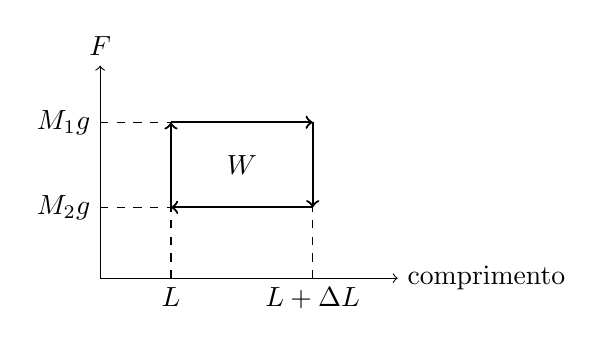
\begin{tikzpicture}[scale=0.9]
\draw[->] (0,0) -- (4.2,0) node[right] {comprimento};
\draw[->] (0,0) -- (0,3) node[above] {$F$};
\draw[thick,->] (1,2.2) -- (3,2.2);
\draw[thick,->] (3,2.2) -- (3,1);
\draw[thick,->] (3,1) -- (1,1);
\draw[thick,->] (1,1) -- (1,2.2);
\draw[dashed] (0,2.2) node[left] {$M_1g$} -- (1,2.2);
\draw[dashed] (0,1) node[left] {$M_2g$} -- (1,1);
\draw[dashed] (1,0) node[below] {$L$} -- (1,1);
\draw[dashed] (3,0) node[below] {$L+\Delta L$} -- (3,1);
\node at (2,1.6) {$W$};
\end{tikzpicture}
\end{center}

\textbf{a)} O trabalho total é a área do retângulo (percorrido no sentido horário, logo $W>0$):
\[
W = (M_1-M_2)\,g\,\alpha L\,\Delta T = (M_1-M_2)\cdot 10\cdot 70\,\alpha L = 700\,\alpha L\,(M_1-M_2)\quad\text{(SI)} .
\]
Unidades: $\text{kg}\cdot\text{m/s}^2\cdot\text{K}^{-1}\cdot\text{m}\cdot\text{K}=\text{J}$. Como $M_1>M_2$, temos $W>0$: a máquina entrega trabalho.

\textbf{b)} A fonte fornece calor apenas na etapa 1. Na etapa 3 o sistema cede calor ao ambiente. Pela 1ª lei, $Q=\Delta U+W$, a energia fornecida se divide em três parcelas:
\begin{itemize}
\item a água (massa $\rho_{\text{H}_2\text{O}}V$) recebe $\rho_{\text{H}_2\text{O}}V c_{\text{H}_2\text{O}}\,\Delta T$;
\item a viga ($n=m/M_{\text{Cu}}$ mols) recebe $\Delta U = n\,c_V\,\Delta T = \dfrac{3Rm}{M_{\text{Cu}}}\,\Delta T$, pela lei de Dulong-Petit (para um sólido, $c_P\simeq c_V$);
\item a viga ainda realiza o trabalho de erguer $M_1$: $M_1 g\,\alpha L\,\Delta T$.
\end{itemize}
Somando:
\[
Q_{\text{abs}} = \Delta T\left(\rho_{\text{H}_2\text{O}}V c_{\text{H}_2\text{O}} + \frac{3Rm}{M_{\text{Cu}}} + M_1 g\alpha L\right).
\]
A eficiência é $\eta = W/Q_{\text{abs}}$. O fator $\Delta T$ se cancela:
\[
\eta = \frac{(M_1-M_2)\,g\,\alpha L}{\rho_{\text{H}_2\text{O}}V c_{\text{H}_2\text{O}} + \dfrac{3Rm}{M_{\text{Cu}}} + M_1 g\alpha L}
= \frac{10\,\alpha L\,(M_1-M_2)}{\rho_{\text{H}_2\text{O}}V c_{\text{H}_2\text{O}} + \dfrac{3Rm}{M_{\text{Cu}}} + 10\,\alpha L M_1}.
\]
O termo $M_1 g\alpha L$ é desprezível diante das capacidades térmicas. Por exemplo, com $\alpha\approx 1{,}7\times10^{-5}\ \text{K}^{-1}$, $L=1$ m e $M_1=20$ kg, ele vale cerca de $3{,}4\times10^{-3}$ J/K, enquanto 1 L de água tem cerca de $4{,}2\times10^{3}$ J/K. Portanto
\[
\eta \simeq \frac{10\,\alpha L\,(M_1-M_2)}{\rho_{\text{H}_2\text{O}}V c_{\text{H}_2\text{O}} + 3Rm/M_{\text{Cu}}} .
\]

\textbf{Verificações.}
\begin{itemize}
\item $\eta$ é adimensional e $\eta\to 0$ quando $M_1\to M_2$.
\item Balanço de energia: o calor cedido no resfriamento é $Q_{\text{ced}}=\Delta T\,(\rho_{\text{H}_2\text{O}}Vc_{\text{H}_2\text{O}}+3Rm/M_{\text{Cu}}+M_2g\alpha L)$, e $Q_{\text{abs}}-Q_{\text{ced}}=W$, como esperado.
\item Ordem de grandeza: com os valores do exemplo, $M_2=10$ kg e uma viga de 1 kg, $\eta\sim 10^{-7}$. Isso é muito menor que o limite de Carnot, $1-\dfrac{293}{363}\approx 0{,}19$, de acordo com a 2ª lei.
\end{itemize}

ANSWER: a) $W=(M_1-M_2)\,g\,\alpha L\,\Delta T = 700\,\alpha L\,(M_1-M_2)$ J (SI); b) $\eta=\dfrac{(M_1-M_2)g\alpha L}{\rho_{\text{H}_2\text{O}}Vc_{\text{H}_2\text{O}}+3Rm/M_{\text{Cu}}+M_1g\alpha L}\simeq\dfrac{10\,\alpha L(M_1-M_2)}{\rho_{\text{H}_2\text{O}}Vc_{\text{H}_2\text{O}}+3Rm/M_{\text{Cu}}}$%
\newpage%
\section*{Questão 6}

\section*{Solução}

\textbf{Convenções e hipóteses.} As lentes são delgadas e estão no ar, e usamos raios paraxiais. Adotamos a convenção de Gauss: $p>0$ para objeto real, $p'>0$ para imagem real (do lado de saída da luz) e $p'<0$ para imagem virtual. Valem
\[
\frac{1}{f}=\frac{1}{p}+\frac{1}{p'},\qquad A=\frac{y'}{y}=-\frac{p'}{p}.
\]
Dados: $f_1=80\ \text{cm}$ (objetiva) e $f_2=5{,}0\ \text{cm}$ (ocular).

\subsection*{a) Comprimento do tubo}
O objeto celeste está praticamente no infinito ($p_1\to\infty$). Logo a objetiva forma uma imagem real $I_1$ no seu foco imagem, isto é, $p_1'=f_1=80\ \text{cm}$.

Pelo enunciado, a imagem final também se forma a grande distância ($p_2'\to\infty$). Para isso, $I_1$ precisa estar no foco objeto da ocular: $p_2=f_2=5{,}0\ \text{cm}$. Os focos das duas lentes coincidem, e o sistema é afocal (ajuste normal). Assim,
\[
L=f_1+f_2=80+5{,}0=85\ \text{cm}.
\]

\subsection*{b) Aumento angular e orientação}
Um feixe vindo do astro chega fazendo um ângulo pequeno $\theta$ com o eixo. A imagem intermediária $I_1$ fica no plano focal comum e tem altura
\[
y_1=-f_1\tan\theta\approx -f_1\,\theta .
\]
O sinal negativo indica que $I_1$ é invertida. Como $I_1$ está no foco da ocular, os raios saem paralelos entre si, sob o ângulo
\[
\theta'\approx \frac{y_1}{f_2}=-\frac{f_1}{f_2}\,\theta .
\]
Portanto
\[
G=\frac{\theta'}{\theta}=-\frac{f_1}{f_2}=-\frac{80}{5{,}0}=-16 .
\]
O aumento angular tem módulo $16$. O sinal negativo mostra que a imagem é \textbf{invertida}: a ocular, que funciona como lupa, não inverte $I_1$, e por isso a imagem final conserva a inversão produzida pela objetiva. Essa imagem final é virtual e fica no infinito.

\subsection*{c) Objeto a $40\ \text{cm}$ da objetiva}
O tubo continua com $L=85\ \text{cm}$, e o objeto real está à frente da objetiva, com $p_1=40\ \text{cm}$.

\textit{Objetiva.} Como $p_1<f_1$,
\[
\frac{1}{p_1'}=\frac{1}{80}-\frac{1}{40}=-\frac{1}{80}\ \Rightarrow\ p_1'=-80\ \text{cm},\qquad A_1=-\frac{-80}{40}=+2 .
\]
$I_1$ é virtual e direita, com o dobro da altura do objeto. Ela fica $80\ \text{cm}$ antes da objetiva, do mesmo lado do objeto.

\textit{Ocular.} $I_1$ funciona como objeto real para a ocular. Sua distância até a ocular é
\[
p_2=L+|p_1'|=85+80=165\ \text{cm}.
\]
Então
\[
\frac{1}{p_2'}=\frac{1}{5{,}0}-\frac{1}{165}=\frac{33-1}{165}=\frac{32}{165}
\ \Rightarrow\ p_2'=\frac{165}{32}\ \text{cm}\approx 5{,}2\ \text{cm},
\]
\[
A_2=-\frac{p_2'}{p_2}=-\frac{165/32}{165}=-\frac{1}{32}.
\]

\textit{Aumento total.}
\[
A=A_1A_2=2\cdot\left(-\frac{1}{32}\right)=-\frac{1}{16}.
\]
Há uma verificação independente: num sistema afocal, o aumento linear é o mesmo para qualquer posição do objeto e vale $-f_2/f_1=-5/80=-1/16$, o que confirma o resultado.

\textbf{Conclusão.} A imagem final é \textbf{real} e se forma $165/32\approx 5{,}2\ \text{cm}$ depois da ocular, do lado do observador; por ser real, poderia ser projetada num anteparo. Ela é \textbf{invertida} ($A<0$) e \textbf{menor} que o objeto: tem $1/16$ da altura dele.

ANSWER: a) $L=85\ \text{cm}$. b) $G=-f_1/f_2=-16$ (módulo 16), imagem invertida. c) Imagem final real, a $165/32\approx 5{,}2\ \text{cm}$ depois da ocular, invertida, com aumento linear $-1/16$; portanto é menor que o objeto (16 vezes menor).%
\newpage%
\section*{Questão 7}

\section*{Solução}

\textbf{Hipóteses.} Cada polarizador é linear. Num polarizador ideal vale a lei de Malus: se a luz chega polarizada linearmente e faz um ângulo $\theta$ com o eixo do polarizador, sai com intensidade $I_{\text{ideal}} = I_{\text{in}}\cos^2\theta$, polarizada ao longo do eixo desse polarizador. Pelo enunciado, a intensidade real após cada polarizador é $x$ vezes a ideal ($0<x\le 1$). Os polarizadores não mudam a seção do feixe, que continua cilíndrico, homogêneo e com o mesmo raio $r$.

\subsection*{a) Intensidade na saída}

\textbf{1º polarizador.} O laser chega com polarização paralela ao eixo, ou seja, $\theta = 0$. O caso ideal deixaria passar $I_0\cos^2 0 = I_0$. Com perdas, a intensidade é
\[
I_1 = x\,I_0 .
\]

\textbf{Polarizadores $2$ a $N+1$.} A luz que sai do polarizador $k$ está polarizada ao longo do eixo dele. O eixo do polarizador seguinte está girado de $\beta$ em relação a esse, portanto
\[
I_{k+1} = x\,I_k\cos^2\beta .
\]
Esse fator aparece $N$ vezes, uma para cada um dos $N$ polarizadores depois do primeiro. Como $\beta = \phi/N$:
\[
I = I_{N+1} = x\,I_0\,\big(x\cos^2\beta\big)^{N}
\;\Longrightarrow\;
\boxed{I = I_0\,x^{N+1}\cos^{2N}\!\left(\frac{\phi}{N}\right)}
\]

\textbf{Verificações.}
\begin{itemize}
\item Com $N=1$ e $x=1$, temos $I = I_0\cos^2\phi$: é a lei de Malus para dois polarizadores.
\item Com $\phi = 0$, temos $I = x^{N+1}I_0$: só sobram as perdas dos $N+1$ polarizadores.
\item Com $x=1$ e $N\to\infty$, vale $\cos^{2N}(\phi/N)\approx \left(1-\frac{\phi^2}{2N^2}\right)^{2N}\to 1$. Ou seja, se cada passo gira pouco o eixo, a polarização gira de $\phi$ quase sem perda. Na prática, porém, o fator $x^{N+1}$ limita o número útil de polarizadores.
\item Como $I\le I_0$, a energia se conserva.
\end{itemize}

\subsection*{b) Raio do feixe}

O feixe é homogêneo, então a intensidade (potência por unidade de área) é uniforme na seção circular de área $\pi r^2$. A potência medida pelo analisador é
\[
P = I\,\pi r^2 \quad\Longrightarrow\quad r = \sqrt{\frac{P}{\pi I}} .
\]
Substituindo o resultado do item (a):
\[
\boxed{r = \sqrt{\dfrac{P}{\pi\,I_0\,x^{N+1}\cos^{2N}\!\left(\phi/N\right)}}}
\]

\textbf{Unidades.} $[P]/[I] = \text{W}/(\text{W/m}^2) = \text{m}^2$, logo $r$ sai em metros.

\textbf{Validade.} A expressão exige $\cos(\phi/N)\neq 0$. Se $\phi/N = 90^\circ$, nenhuma luz sai do sistema ($P=0$) e não é possível obter o raio dessa forma.

ANSWER: a) $I = I_0\,x^{N+1}\cos^{2N}(\phi/N)$; b) $r = \sqrt{\dfrac{P}{\pi I_0\,x^{N+1}\cos^{2N}(\phi/N)}}$%
\newpage%
\section*{Questão 8}

\section*{Solução}

\textbf{Dados (SI):} $m=100\ \text{g}$, $c=2{,}0\ \text{J/(g}\,^\circ\text{C)}$, $\Delta\theta=30\ ^\circ\text{C}$, $q=2\ \text{Ah}=7200\ \text{C}$, $\varepsilon=5{,}0\ \text{V}$, $T_{\text{total}}=20\ \text{min}=1200\ \text{s}$, $n=20\ \text{espiras/cm}=2000\ \text{m}^{-1}$, $r=5\times10^{-3}\ \text{m}$, $\ell=2\times10^{-2}\ \text{m}$ (logo $N=n\ell=40$ espiras), $\Delta I=14\ \text{A}$.

\subsection*{a) Potência média mínima}

Pela conservação da energia, a energia entregue pelo carregador deve, no mínimo, cobrir dois termos.

\emph{Energia armazenada na bateria} (carga $q$ sob a tensão $\varepsilon$):
\[
E_{\text{bat}}=q\,\varepsilon=(2\ \text{A}\cdot 3600\ \text{s})(5{,}0\ \text{V})=36000\ \text{J}.
\]

\emph{Calor que aqueceu o aparelho:}
\[
Q=m\,c\,\Delta\theta=100\cdot 2{,}0\cdot(50-20)=6000\ \text{J}.
\]

Outras perdas (calor cedido ao ambiente, dissipação no próprio carregador etc.) só aumentariam a energia necessária. Por isso o valor mínimo corresponde a supor que essas são as únicas parcelas:
\[
P_{\min}=\frac{E_{\text{bat}}+Q}{T_{\text{total}}}=\frac{36000+6000}{1200}=35\ \text{W}.
\]
(Verificação: a corrente média de carga é $7200/1200=6\ \text{A}$, o que dá $30\ \text{W}$ para a bateria e $5\ \text{W}$ dissipados em calor.)

\subsection*{b) Máximo $\Delta t$}

\emph{Indutância.} No modelo de solenoide ideal, $B=\mu_0 n I$ no interior. O fluxo total no próprio solenoide é $N\,B\,\pi r^2$, o que dá
\[
L=\mu_0 n^2 \pi r^2 \ell=(4\pi\times10^{-7})(2000)^2\,\pi\,(5\times10^{-3})^2(2\times10^{-2})=8\pi^2\times10^{-7}\ \text{H}\approx 7{,}9\times10^{-6}\ \text{H}.
\]
Para duas bobinas, a indutância mútua satisfaz $M\le\sqrt{L_1L_2}=L$, com igualdade apenas no acoplamento perfeito (todo o fluxo de uma bobina atravessa a outra). O modelo ideal também superestima o campo de um solenoide real curto. Logo $M=L$ é o maior valor possível.

\emph{Lei de Faraday--Neumann.} A corrente varia linearmente, então $di/dt=\Delta I/\Delta t$ é constante e a f.e.m. induzida na bobina do celular também é constante:
\[
|\varepsilon|=M\,\frac{\Delta I}{\Delta t}\quad\Longrightarrow\quad \Delta t=\frac{M\,\Delta I}{\varepsilon}\le\frac{L\,\Delta I}{\varepsilon}.
\]
Portanto
\[
\Delta t_{\max}=\frac{8\pi^2\times10^{-7}\cdot 14}{5{,}0}=2{,}24\,\pi^2\times10^{-6}\ \text{s}\approx 2{,}2\times10^{-5}\ \text{s}.
\]

\emph{Verificação energética.} No acoplamento perfeito de bobinas idênticas, a bobina do carregador também tem f.e.m. $\varepsilon$ durante a rampa. A potência que ela fornece é então $\varepsilon\,i(t)$, com $i$ variando linearmente de $0$ a $14\ \text{A}$. Sua média é
\[
\bar P=\varepsilon\,\frac{0+14}{2}=5{,}0\cdot 7=35\ \text{W},
\]
exatamente a potência mínima do item (a).

De modo equivalente, cada ciclo transfere no máximo a energia magnética $\tfrac12 L I_{\max}^2=\tfrac12\,(8\pi^2\times10^{-7})(14)^2\approx 7{,}7\times10^{-4}\ \text{J}$. Com $P_{\min}=35\ \text{W}$, isso também limita
\[
\Delta t\le\frac{\tfrac12 L I_{\max}^2}{P_{\min}}\approx\frac{7{,}74\times10^{-4}}{35}\approx 2{,}2\times10^{-5}\ \text{s}.
\]
Os dois caminhos dão o mesmo resultado. A ordem de grandeza (dezenas de microssegundos, ou seja, frequência de dezenas de kHz) é típica de carregadores indutivos.

ANSWER: a) $P_{\min}=35\ \text{W}$; \quad b) $\Delta t_{\max}=\dfrac{\mu_0 n^2\pi r^2\ell\,\Delta I}{\varepsilon}=2{,}24\,\pi^2\times10^{-6}\ \text{s}\approx 2{,}2\times10^{-5}\ \text{s}$%
\newpage%
\section*{Questão 9}

\section*{Solução}

\textbf{Hipóteses.} A luz solar chega como ondas planas (raios paralelos) em incidência normal sobre a grade. Como o espaçamento $d$ entre ranhuras é muito menor que a altura $H = 20\ \text{cm}$, os raios que saem de ranhuras vizinhas rumo a um mesmo ponto do solo são praticamente paralelos (regime de Fraunhofer). O \emph{ponto central} é o pé da perpendicular à grade traçada até o solo, onde está o máximo central ($m=0$) de todas as cores, que se somam e dão luz branca.

\textbf{Condição de máximo.} Com incidência normal, a diferença de caminho entre raios de ranhuras vizinhas que saem com ângulo $\theta$ em relação à normal é $d\sin\theta$. Há interferência construtiva quando
\[
d\sin\theta = m\lambda, \qquad m = 0, 1, 2, \dots
\]
Para a primeira ordem, $m = 1$.

\textbf{Geometria.} Um máximo que sai da grade com ângulo $\theta$ chega ao solo a uma distância $x$ do ponto central dada por
\[
\tan\theta = \frac{x}{H}.
\]
Aqui o ângulo não é pequeno, então \emph{não} vale usar $\sin\theta \approx \tan\theta$. Por isso usamos as relações trigonométricas exatas.

\subsection*{a) Distância entre as ranhuras}

Para o laranja, $x_L = H = 20\ \text{cm}$. Então
\[
\tan\theta_L = \frac{20}{20} = 1 \;\Rightarrow\; \theta_L = 45^\circ, \qquad \sin\theta_L = \frac{\sqrt{2}}{2}.
\]
Substituindo na condição de máximo com $m=1$:
\[
d = \frac{\lambda_L}{\sin\theta_L} = \frac{600\ \text{nm}}{\sqrt{2}/2} = 600\sqrt{2}\ \text{nm} \approx 849\ \text{nm} \approx 8{,}5\times 10^{-7}\ \text{m}.
\]
Isso equivale a cerca de $1{,}2\times 10^{3}$ ranhuras por milímetro, valor típico de uma grade comercial.

\subsection*{b) Primeiro máximo do violeta}

A grade é a mesma, com $d = 600\sqrt{2}\ \text{nm}$. Para $\lambda_V = 400\ \text{nm}$ e $m = 1$:
\[
\sin\theta_V = \frac{\lambda_V}{d} = \frac{400}{600\sqrt{2}} = \frac{\sqrt{2}}{3} \approx 0{,}471,
\]
\[
\cos\theta_V = \sqrt{1 - \frac{2}{9}} = \frac{\sqrt{7}}{3}, \qquad \tan\theta_V = \frac{\sqrt{2}}{\sqrt{7}} = \sqrt{\frac{2}{7}}.
\]
Logo,
\[
x_V = H\tan\theta_V = 20\sqrt{\frac{2}{7}}\ \text{cm} = \frac{20\sqrt{14}}{7}\ \text{cm} \approx 10{,}7\ \text{cm}.
\]

\textbf{Verificações.}
\begin{itemize}
\item O violeta tem comprimento de onda menor, então é menos desviado: $\theta_V \approx 28^\circ < 45^\circ$ e $x_V < x_L$, como esperado.
\item Se tivéssemos usado a aproximação $x \propto \lambda$ (ângulos pequenos), obteríamos $x_V = \tfrac{2}{3}\cdot 20 \approx 13{,}3\ \text{cm}$. Esse valor está errado, porque $\theta_L = 45^\circ$ não é um ângulo pequeno.
\item O máximo de 2ª ordem do violeta tem $\sin\theta = 800/849 \approx 0{,}94$, ou seja, $\theta \approx 70^\circ$. Ele cai longe e não se confunde com o de 1ª ordem.
\end{itemize}

ANSWER: a) $d = 600\sqrt{2}\ \text{nm} \approx 8{,}5\times 10^{-7}\ \text{m}$; b) $x_V = 20\sqrt{2/7}\ \text{cm} = \frac{20\sqrt{14}}{7}\ \text{cm} \approx 10{,}7\ \text{cm}$.%
\newpage%
\section*{Questão 10}

\section*{Solução}

\textbf{Hipóteses.} Adotamos o referencial inercial $S$ da Terra (o Sol e a Terra têm velocidade desprezível em comparação com $c$). A origem é a fronteira do sistema Solar, $x=0$ em $t=t_0=0$, e o eixo $x$ aponta para Sirius, que está em repouso em $S$, a $D=8{,}6$ anos-luz (a.l.). Usamos anos e anos-luz, de modo que $c=1$ a.l./ano. As duas naves partem de $x=0$ no mesmo instante $t_0$. Como as trajetórias são paralelas e a separação lateral entre elas é desprezível, as partidas formam praticamente um único evento $O$. Além disso, uma separação puramente transversal não altera a simultaneidade em referenciais que se movem ao longo de $x$: pela transformação de Lorentz, $t'=\gamma(t-vx/c^2)=0$ para as duas partidas. O sinal é eletromagnético e se propaga com velocidade $c$ em qualquer referencial inercial (2º postulado).

\textbf{a)} Movimentos uniformes em $S$:
\[
x_1(t)=0{,}8\,c\,t,\qquad x_2(t)=0{,}6\,c\,t .
\]
\emph{Chegada da nave 1 a Sirius} (evento $E$ de emissão):
\[
t_E=\frac{D}{v_1}=\frac{8{,}6\ \text{a.l.}}{0{,}8\,c}=10{,}75\ \text{anos},\qquad x_E=8{,}6\ \text{a.l.}
\]
Nesse instante, a nave 2 está em $x_2(t_E)=0{,}6\cdot 10{,}75=6{,}45$ a.l., ou seja, ainda a $8{,}6-6{,}45=2{,}15$ a.l. de Sirius.

\emph{Recepção} (evento $R$): o sinal volta, $x_s(t)=D-c\,(t-t_E)$, e encontra a nave 2 quando $x_s(t_R)=x_2(t_R)$:
\[
D-c\,(t_R-t_E)=0{,}6\,c\,t_R\;\Longrightarrow\; t_R=\frac{D/c+t_E}{1{,}6}=\frac{8{,}6+10{,}75}{1{,}6}=\frac{19{,}35}{1{,}6}=12{,}09375\ \text{anos}.
\]
Verificação: de $t_E$ até $t_R$ a distância de $2{,}15$ a.l. é fechada com velocidade relativa $c+0{,}6c=1{,}6c$ (medida em $S$), o que leva $2{,}15/1{,}6=1{,}34375$ ano; e $10{,}75+1{,}34375=12{,}09375$ anos. Portanto
\[
\Delta t_{\text{Terra}}=\frac{387}{32}\ \text{anos}\approx 12{,}1\ \text{anos}.
\]
Esse é o intervalo de \emph{coordenada} em $S$. Não inclui o tempo que alguma informação levaria para chegar até a Terra.

\textbf{b)} Os eventos $O$ e $R$ acontecem ambos na nave 2, que tem velocidade constante. O intervalo pedido é, então, o tempo próprio da nave 2 (dilatação temporal):
\[
\gamma_2=\frac{1}{\sqrt{1-0{,}6^2}}=\frac{1}{0{,}8}=1{,}25,\qquad
\Delta\tau_2=\frac{\Delta t_{\text{Terra}}}{\gamma_2}=0{,}8\cdot 12{,}09375=9{,}675\ \text{anos}.
\]

\emph{Conferência no referencial $S'$ da nave 2.} Aplicando a transformação de Lorentz ao evento $E$:
\[
t'_E=\gamma_2\left(t_E-\frac{v_2x_E}{c^2}\right)=1{,}25\,(10{,}75-0{,}6\cdot 8{,}6)=6{,}9875\ \text{anos},\qquad
x'_E=\gamma_2\,(x_E-v_2t_E)=1{,}25\,(8{,}6-6{,}45)=2{,}6875\ \text{a.l.}
\]
Em $S'$ a nave 2 está parada em $x'=0$, e o sinal leva $2{,}6875$ anos para chegar até ela. Assim, $\Delta\tau_2=6{,}9875+2{,}6875=9{,}675$ anos, o mesmo resultado.

\textbf{Coerência.} $\Delta\tau_2<\Delta t_{\text{Terra}}$, como se espera para um relógio em movimento em relação a $S$. Ambos os valores superam o mínimo $D/c=8{,}6$ anos que a luz levaria para ir até Sirius. O caso clássico daria o mesmo $t_R$ em $S$, mas sem dilatação: $\Delta\tau_2=\Delta t$.

ANSWER: a) $\Delta t_{\text{Terra}}=\dfrac{387}{32}\ \text{anos}=12{,}09375\ \text{anos}\approx 12{,}1\ \text{anos}$; b) $\Delta\tau_2=\dfrac{387}{40}\ \text{anos}=9{,}675\ \text{anos}\approx 9{,}7\ \text{anos}$.%
\newpage%
\section*{Apêndice: parecer do avaliador}%
\subsection*{Questão 1: nota 9,2 (aprovada, rodada 1 de 1)}%
\textbf{Resposta da resolução às cegas do avaliador:} a) R\_min = v$^2$(1 - $\mu$ tg $\theta$) / {[}g (tg $\theta$ + $\mu$){]} = v$^2$(cos $\theta$ - $\mu$ sen $\theta$) / {[}g (sen $\theta$ + $\mu$ cos $\theta$){]} = v$^2$ / {[}g tg($\theta$ + arctg $\mu$){]}. Vale se $\mu$ tg $\theta$ < 1; se $\mu$ $\geq$ cotg $\theta$, não há raio mínimo. No limite, a roda interna está na iminência de perder o contato e a roda externa na iminência de escorregar, com o atrito ao longo da geratriz, para baixo e para o centro da curva.\newline%
\newline%
b) R\_min = v$^2$/(g tg $\theta$) = v$^2$ cotg $\theta$ / g. No limite, N? = 0 e N? = Mg/cos $\theta$.\newline%
\newline%
c) R\_min = v$^2$/($\mu$ g).\newline%
\newline%
Nenhuma das respostas depende de M.\par %
As respostas finais coincidem com a referência nos três itens e estão corretas: (a) R\_min = v$^2$(1-$\mu$ tg $\theta$)/{[}g(tg $\theta$+$\mu$){]} = v$^2$/{[}g tg($\theta$+arctg $\mu$){]}, válida para $\mu$ tg $\theta$ < 1; (b) R\_min = v$^2$/(g tg $\theta$); (c) R\_min = v$^2$/($\mu$g). Conferi em python3 que as três formas de (a) são equivalentes e que a varredura dos cones de atrito reproduz R\_min, por exemplo 102,54 m para $\theta$ = 10$^\circ$, $\mu$ = 0,2 e v = 20 m/s. A figura original confirma a leitura do candidato: o raio da roda é maior junto ao eixo, a normal é inclinada de $\theta$ em relação à vertical e aponta para o meio do eixo, e é a roda interna que perde o contato. O candidato tratou todas as armadilhas: direção correta da normal; item (b) como desigualdade, com N$_{2}$ explícita e a condição N$_{2}$ $\geq$ 0; atrito da roda externa para baixo e para o centro da curva; indeterminação estática resolvida pelo cone de atrito, um tratamento rigoroso e elegante; condição de validade $\mu$ tg $\theta$ < 1, com o caso autotravante; item (c) com normais verticais, centrípeta só pelo atrito e interpretação como escorregamento lateral; hipóteses do modelo (R muito maior que as dimensões, sem balanço de torques, v constante); e verificações (limites $\mu$$\to$0 e $\theta$$\to$0, dimensão, R\_a < R\_b e R\_a < R\_c). As falhas são todas menores. A suficiência para R > R\_min não foi demonstrada. Falta o passo que mostra que a igualdade exige N$_{2}$ = 0 quando $\theta$ > 0. Há pequenas imprecisões de redação e a comparação com a pista sobrelevada no item (b) pode confundir. É uma resolução que serviria quase sem alterações como gabarito comentado.%
\begin{itemize}%
\item%
{[}minor{]} Item (a): o argumento do cone de atrito prova só a necessidade, isto é, que se R < R\_min não existe distribuição admissível de forças. A suficiência não é demonstrada. A conferência no limiar mostra que em R = R\_min existe uma solução com N$_{2}$ = 0, mas o texto não mostra que para todo R > R\_min existe uma solução com N$_{2}$ > 0, que é o que garante que nenhuma roda perde o contato. Bastaria uma frase: os dois cones somados cobrem todas as direções com ângulo em {[}-$\theta$-$\varphi$, $\theta$+$\varphi${]}, então qualquer direção interior é obtida com as duas forças não nulas.%
\item%
{[}minor{]} Item (a): o texto diz que 'a igualdade exige que toda a força venha da roda externa', mas pula um passo. Para a roda 2 atingir a cota seria preciso $\alpha$$_{2}$ = $\theta$+$\varphi$, o que é impossível se $\theta$ > 0, já que $\alpha$$_{2}$ $\leq$ -$\theta$+$\varphi$. Logo Y$_{2}$ = 0 e N$_{2}$ = 0. Esse passo devia aparecer, inclusive para mostrar que em $\theta$ = 0 a igualdade não força N$_{2}$ = 0, o que é coerente com o item (c).%
\item%
{[}minor{]} Item (a), redação: 'Para R menor, não existe distribuição de forças com N$_{2}$ $\geq$ 0'. Na verdade, abaixo de R\_min não existe distribuição admissível nenhuma, e a condição N$_{2}$ $\geq$ 0 é sempre obrigatória. Também faltou dizer fisicamente o que acontece: a roda interna levanta ou a roda externa sobe no trilho.%
\item%
{[}minor{]} Item (b): o comentário 'é o mesmo resultado de uma curva sem atrito com inclinação $\theta$' não avisa que, na pista sobrelevada, R = v$^2$/(g tg $\theta$) é o único raio possível, enquanto aqui é só uma cota inferior e serve qualquer R $\geq$ R\_min. A desigualdade foi deduzida corretamente, mas o comentário pode confundir o leitor.%
\item%
{[}minor{]} O texto acrescenta a hipótese 'resistências desprezadas', que não está no enunciado, para dizer que não há atrito longitudinal. É razoável, mas deveria aparecer explicitamente como hipótese adicional.%
\end{itemize}%
\subsection*{Questão 2: nota 9,0 (aprovada, rodada 1 de 1)}%
\textbf{Resposta da resolução às cegas do avaliador:} **a)** As normais são perpendiculares ao plano. Seja W = (M + m + m\_C)g.\newline%
N\_A = g cos$\theta$ $\cdot$ {[}M(L/2 - d) + m(L - a - d) + m\_C(b - d){]} / (L - 2d) = g cos$\theta$ $\cdot$ {[}M/2 + (m(L - a - d) + m\_C(b - d))/(L - 2d){]}\newline%
N\_B = g cos$\theta$ $\cdot$ {[}M(L/2 - d) + m(a - d) + m\_C(L - b - d){]} / (L - 2d) = g cos$\theta$ $\cdot$ {[}M/2 + (m(a - d) + m\_C(L - b - d))/(L - 2d){]}\newline%
Conferência: N\_A + N\_B = (M + m + m\_C) g cos$\theta$. A resposta vale com espessura e altura dos apoios desprezíveis, com L > 2d e com N\_A, N\_B $\geq$ 0.\newline%
\newline%
**b)** As forças de atrito sobre a barra apontam plano acima. Só a soma sai das equações de equilíbrio:\newline%
f\_A + f\_B = (M + m + m\_C) g sin$\theta$.\newline%
A divisão entre A e B é estaticamente indeterminada: os dois atritos ficam sobre a mesma reta e não dão torque um em relação ao apoio do outro.\newline%
Supondo o mesmo coeficiente nos dois apoios e atrito proporcional à normal (é o caso de atrito mínimo, $\mu$\_mín = tan$\theta$):\newline%
f\_A = N\_A tan$\theta$ = g sin$\theta$ $\cdot$ {[}M(L/2 - d) + m(L - a - d) + m\_C(b - d){]} / (L - 2d)\newline%
f\_B = N\_B tan$\theta$ = g sin$\theta$ $\cdot$ {[}M(L/2 - d) + m(a - d) + m\_C(L - b - d){]} / (L - 2d)\newline%
Outra hipótese aceitável, desde que declarada: apoios idênticos e divisão igual, f\_A = f\_B = (M + m + m\_C) g sin$\theta$ / 2.\par %
Conferi o enunciado com o PDF (p. 3). A transcrição está fiel: a é medido a partir da extremidade inferior, b a partir da superior, e os apoios ficam a uma distância d de cada ponta.\newline%
\newline%
**Item a.** A resposta do candidato coincide com a minha referência:\newline%
{-} N\_A = g cos$\theta${[}M/2 + (m(L-a-d) + m\_C(b-d))/(L-2d){]}\newline%
{-} N\_B = g cos$\theta${[}M/2 + (m(a-d) + m\_C(L-b-d))/(L-2d){]}\newline%
\newline%
Conferi numericamente em python, com valores aleatórios, a soma das forças perpendiculares e o torque em relação à extremidade. Os dois resíduos dão cerca de 1e{-}15.\newline%
\newline%
**Item b.**\newline%
{-} A soma f\_A + f\_B = (M+m+m\_C) g sin$\theta$ está correta, e os atritos sobre a barra apontam rampa acima.\newline%
{-} O candidato reconhece explicitamente o hiperestatismo: os atritos são colineares, então só a soma é determinada.\newline%
{-} Para separar os dois atritos, adota a hipótese de mesmo $\mu$ e atrito mínimo, e deduz corretamente que $\mu$ $\geq$ tan$\theta$.\newline%
{-} No caso limite, mostra bem por que cada parcela atinge seu máximo: a soma vale $\mu$(N\_A+N\_B) e cada f\_i $\leq$ $\mu$N\_i. Daí f\_i = N\_i tan$\theta$, idêntico à referência.\newline%
{-} A conferência f\_A + f\_B = (M+m+m\_C) g sin$\theta$ também passou.\newline%
\newline%
**Armadilhas.** Todas foram tratadas:\newline%
{-} braços de alavanca medidos a partir dos apoios, com g cos$\theta$;\newline%
{-} contrapeso em x = L - b;\newline%
{-} denominador L - 2d;\newline%
{-} hipótese de espessura e altura dos apoios desprezíveis, declarada;\newline%
{-} normais perpendiculares ao plano, com soma (M+m+m\_C) g cos$\theta$;\newline%
{-} validade N\_i $\geq$ 0 e papel do contrapeso;\newline%
{-} hiperestatismo do item b;\newline%
{-} hipótese declarada para dividir os atritos;\newline%
{-} sentido do atrito;\newline%
{-} $\mu$\_mín = tan$\theta$, independente de a, b e d.\newline%
\newline%
Há boas verificações: simetria, caso a = d, caso $\theta$ = 0 e unidades. A 3ª lei aparece no item a.\newline%
\newline%
**Por que não 10.** Há três falhas menores:\newline%
{-} notação estranha ('peso Pg');\newline%
{-} não diz que, para $\mu$ > tan$\theta$, a divisão continua indeterminada, nem cita a divisão igual como alternativa;\newline%
{-} falta um pouco de detalhe na montagem das equações de torque.\newline%
\newline%
Mesmo assim, é uma resolução de padrão de gabarito comentado. Nota 9.%
\begin{itemize}%
\item%
{[}minor{]} Notação: 'Cada peso \$Pg\$' usa P como símbolo de massa, e P costuma indicar peso. O certo seria 'cada massa \$\textbackslash{}mu\_i\$ tem peso \$\textbackslash{}mu\_i g\$' ou falar diretamente em Mg, mg e m\_Cg.%
\item%
{[}minor{]} No item b, os valores f\_i = N\_i tan$\theta$ aparecem em destaque como resposta, mas só são únicos no caso limite $\mu$ = tan$\theta$. A resolução diz que a estática determina apenas a soma, mas não diz que, para $\mu$ > tan$\theta$, qualquer divisão com f\_i $\leq$ $\mu$N\_i e soma fixa é admissível. Também não menciona a alternativa da divisão igual, (M+m+m\_C)g sin$\theta$/2. Uma frase deixaria claro que a escolha é uma hipótese de fechamento, e não uma consequência das equações.%
\item%
{[}minor{]} As equações de torque em A e em B aparecem já na forma final. Faltam o sentido adotado como positivo e a frase 'braço = distância ao longo da barra, com a componente g cos$\theta$ do peso'. O resultado está certo, mas um gabarito comentado mostraria essa passagem. A hipótese de barra fina está declarada antes.%
\end{itemize}%
\subsection*{Questão 3: nota 9,0 (aprovada, rodada 1 de 1)}%
\textbf{Resposta da resolução às cegas do avaliador:} a) A componente radial da reação do pivô fica ao longo da haste. Tomando como positivo o sentido do centro de massa para o pivô:\newline%
R = M{[}g cos$\theta$ + $\omega$$^2$(L/2 - a){]} = M{[}g cos$\theta$ + $\omega$$^2$(L - 2a)/2{]}.\newline%
Se R < 0, o pivô empurra a haste para fora. Vetorialmente, com r? = (sin$\theta$, -cos$\theta$) unitário do pivô para a ponta longa: N\_r = -M{[}g cos$\theta$ + $\omega$$^2$(L/2 - a){]} r?.\newline%
\newline%
b) R = 0 $\Leftrightarrow$ cos$\theta$ = -$\omega$$^2$(L - 2a)/(2g), ou seja, $\theta$ = arccos{[}-$\omega$$^2$(L - 2a)/(2g){]} = $\pi$ - arccos{[}$\omega$$^2$(L - 2a)/(2g){]}.\newline%
{-} Para a < L/2, isso dá 90$^\circ$ < $\theta$ $\leq$ 180$^\circ$: o centro de massa fica acima do pivô.\newline%
{-} Por simetria, -$\theta$ também serve.\newline%
{-} A massa M não aparece no resultado.\newline%
{-} Só existe solução se $\omega$$^2$(L - 2a) $\leq$ 2g.\newline%
{-} Para a = L/2, o resultado é $\theta$ = 90$^\circ$, qualquer que seja $\omega$.\par %
Conferi o enunciado original (p. 4), que confere com a transcrição. As respostas finais do candidato coincidem com as da referência nos dois itens. Também conferi numericamente: montei a dinâmica completa com $\alpha$ = -Mgd$\cdot$sin$\theta$/I\_O, calculei N = M$\cdot$a\_CM - M$\cdot$g e projetei em r?, para vários ($\theta$, $\omega$). O resultado bate com -F\_r até a precisão de máquina. Para L = 1,5, a = 0,3 e $\omega$ = 2, a fórmula do item b dá $\theta$ $\approx$ 100,37$^\circ$, com F\_r = 0.\newline%
\newline%
**Item a.** A resolução está correta e bem justificada:\newline%
{-} d = L/2 - a está certo;\newline%
{-} o versor r? = (sin$\theta$, -cos$\theta$) está definido explicitamente;\newline%
{-} usa o teorema do CM num referencial inercial, sem força centrífuga;\newline%
{-} projeta o peso com o sinal correto (+Mg$\cdot$cos$\theta$);\newline%
{-} observa que $\alpha$ não entra na direção radial, então não usa momento de inércia nem energia;\newline%
{-} define que o sentido positivo é para o pivô;\newline%
{-} dá a forma vetorial correta;\newline%
{-} faz verificações de unidade e dos casos $\theta$ = 0, $\omega$ = 0 e a = L/2.\newline%
\newline%
**Item b.** $\theta$ = arccos{[}$\omega$$^2$(2a - L)/(2g){]} está certo. A discussão também é boa:\newline%
{-} diz que cos$\theta$ < 0, logo 90$^\circ$ < $\theta$ $\leq$ 180$^\circ$, e interpreta fisicamente;\newline%
{-} dá a condição de existência $\omega$ $\leq$ $\surd$(2g/(L - 2a));\newline%
{-} mostra o limite $\omega$ $\to$ 0;\newline%
{-} nota que o resultado independe de M;\newline%
{-} justifica por que qualquer par ($\theta$, $\omega$) é possível, escolhendo a energia.\newline%
\newline%
**Falhas.** São poucas e menores:\newline%
{-} F\_r é chamado de 'módulo' e dito 'orientado para o pivô' sem a ressalva de que pode ser negativo para $\theta$ > 90$^\circ$. A forma vetorial, porém, está certa.\newline%
{-} Falta citar a solução simétrica -$\theta$.\newline%
{-} O caso a = L/2 não é comentado no item b.\newline%
\newline%
Todas as armadilhas principais foram evitadas: distância do CM, sinal do peso, referencial inercial, não usar I nem energia no item a, componente ao longo da haste e não nos eixos, cosseno negativo e condição de existência no item b. Com um pequeno ajuste de redação, a resolução serviria de gabarito comentado.%
\begin{itemize}%
\item%
{[}minor{]} Item a: a fórmula F\_r = M{[}$\omega$$^2$(L-2a)/2 + g cos$\theta${]} aparece descrita como valor 'em módulo e orientada para o pivô'. Isso falha quando o colchete é negativo, o que ocorre para $\theta$ > 90$^\circ$ com |g cos$\theta$| > $\omega$$^2$d. Exemplo: $\theta$ = 2,0 rad, $\omega$ = 2,5 rad/s, L = 1,5, a = 0,3 dá F\_r $\approx$ -2,70 N. Nesse caso o pivô empurra a haste para fora, e F\_r não é um módulo. A forma vetorial F\_r(-sin$\theta$, cos$\theta$) está correta para qualquer $\theta$. O texto deveria chamar F\_r de componente algébrica, positiva quando aponta para o pivô e negativa quando aponta para fora. A resposta final ('dirigida para o pivô') também deveria trazer essa ressalva.%
\item%
{[}minor{]} Item b: falta dizer que -$\theta$ também é solução, com a haste do outro lado da vertical, porque cos(-$\theta$) = cos$\theta$. O arccos só devolve o ângulo em {[}0, $\pi${]}. Uma frase sobre a simetria resolveria.%
\item%
{[}minor{]} Item b: o caso a = L/2 ($\theta$ = 90$^\circ$ para qualquer $\omega$) não é discutido explicitamente. Ele aparece de forma implícita na verificação do item a e na fórmula. Também não se comenta que o enunciado pede a resposta 'em função de M', embora o resultado não dependa de M. O candidato diz que o resultado independe de M, mas não aponta o conflito com o enunciado. É detalhe de completude.%
\end{itemize}%
\subsection*{Questão 4: nota 9,5 (aprovada, rodada 1 de 1)}%
\textbf{Resposta da resolução às cegas do avaliador:} a) Com o CM das partes sobre a elipse, o CM fica em (4a/5, $\pm$3b/5). Então y$_{2}$ = 2b (CM em (4a/5, 3b/5)) ou y$_{2}$ = -4b (CM em (4a/5, -3b/5)).\newline%
\newline%
b) O mínimo ocorre com a estrela no foco (c, 0) mais próximo das partes, c = $\surd$(a$^2$ - b$^2$), e com y$_{2}$ = 2b:\newline%
U\_min = -(GMm/5){[}16/$\surd$((3a - 4c)$^2$ + b$^2$) + 1/$\surd$((a - c)$^2$ + 4b$^2$){]} - 16Gm$^2$/(25$\surd$(a$^2$ + 49b$^2$)).\newline%
Como M ? m, o último termo (interação m$_{1}$--m$_{2}$) é desprezível:\newline%
U\_min $\approx$ -(GMm/5){[}16/$\surd$(25a$^2$ - 24a$\surd$(a$^2$-b$^2$) - 15b$^2$) + 1/$\surd$(2a$^2$ - 2a$\surd$(a$^2$-b$^2$) + 3b$^2$){]}.\par %
O enunciado transcrito confere com o PDF (p. 5). A resolução do candidato coincide com a minha referência nos dois itens.\newline%
\newline%
(a) Ele diz explicitamente a hipótese central: a separação vem de forças internas e o CM fica sobre a elipse, com a ressalva sobre a idealização. Calcula as massas certas (m$_{1}$ = 4m/5, m$_{2}$ = m/5) e o CM (4a/5, (b+y$_{2}$)/5), e encontra as duas soluções y$_{2}$ = 2b ou y$_{2}$ = -4b, ambas declaradas compatíveis.\newline%
\newline%
(b) Ele escreve U com os três pares de interação e interpreta 'menor' como 'mais negativa'. Prova que o foco (+c, 0) reduz r$_{1}$ e r$_{2}$ ao mesmo tempo, porque x > 0 implica (x-c)$^2$ < (x+c)$^2$. Também mostra que y$_{2}$ = 2b reduz r$_{2}$ e d (r$_{1}$ não depende de y$_{2}$). Assim, não precisa comparar valores numéricos entre configurações. As distâncias estão corretas e c = $\surd$(a$^2$-b$^2$) está explicitado. As formas alternativas dos radicandos, 25a$^2$-24ac-15b$^2$ e 2a$^2$-2ac+3b$^2$, estão certas. O termo m$_{1}$--m$_{2}$ aparece na resposta exata e depois é desprezado com justificativa.\newline%
\newline%
Conferi em Python, para vários pares (a, b), inclusive a = b:\newline%
{-} o CM (4a/5, $\pm$3b/5) satisfaz a equação da elipse;\newline%
{-} entre as 4 combinações, o mínimo é sempre foco (+c, 0) com y$_{2}$ = 2b;\newline%
{-} a fórmula fechada coincide com o cálculo direto. Exemplo: a = 1, b = 0,6 dá -5224,19 com G = 1, M = 1000, m = 1;\newline%
{-} as identidades dos radicandos valem.\newline%
\newline%
A resolução trata todas as armadilhas: hipótese do CM, duas raízes de y$_{2}$, estrela no foco e não no centro, escolha do foco, sinal da energia, não usar massa pontual no CM, massas corretas, termo de interação e caso circular. Só há imprecisões menores de redação: a menção a 'sistema ligado', a referência no infinito não declarada e a ordem de grandeza do termo m$_{1}$--m$_{2}$ um pouco vaga. É uma resolução de nível gabarito comentado.%
\begin{itemize}%
\item%
{[}minor{]} Na verificação de sinal, o candidato escreve que U\_min < 0 'como deve ser para um sistema ligado'. U < 0 decorre só da escolha da referência no infinito: a energia potencial gravitacional é sempre negativa, mesmo num sistema não ligado. Depois da fragmentação, nem se sabe se as partes continuam ligadas. Bastava dizer que U < 0 porque a referência está no infinito.%
\item%
{[}minor{]} A referência U = 0 no infinito não é dita explicitamente; ela fica implícita no uso de -GMm/r. Para o rigor de um gabarito, convém declará{-}la, porque a interpretação de 'menor energia' como 'mais negativa' depende dela.%
\item%
{[}minor{]} A frase 'o termo m$_{1}$--m$_{2}$ é da ordem de m/M em relação aos outros' é um pouco imprecisa. A razão é (m/M)$\cdot$(r/d), e aqui d e r são da mesma ordem, então a conclusão vale. Mesmo assim, uma linha justificando que d e r são comparáveis deixaria o argumento completo. O candidato manteve o termo na resposta exata, o que é a escolha mais segura.%
\item%
{[}minor{]} O teste do caso circular confere só r$_{1}$ e r$_{2}$, não o valor de U\_min nem o de d. É uma verificação parcial, sem impacto na correção.%
\end{itemize}%
\subsection*{Questão 5: nota 9,0 (aprovada, rodada 1 de 1)}%
\textbf{Resposta da resolução às cegas do avaliador:} a) W = (M$_{1}$ - M$_{2}$)g$\cdot$$\alpha$L$\cdot$$\Delta$T, com $\Delta$T = 70 K, ou seja, W = 70$\alpha$L(M$_{1}$ - M$_{2}$)g = 700$\alpha$L(M$_{1}$ - M$_{2}$) J no SI. É o trabalho líquido realizado pela viga: ela ergue M$_{1}$ por $\Delta$L = 70$\alpha$L e deixa M$_{2}$ descer o mesmo $\Delta$L.\newline%
\newline%
b) $\eta$ = W/Q\_fonte, com Q\_fonte = 70($\rho$\_\{H$_{2}$O\}Vc\_\{H$_{2}$O\} + 3Rm/M\_Cu). Assim, $\eta$ = (M$_{1}$ - M$_{2}$)g$\alpha$L / ($\rho$\_\{H$_{2}$O\}Vc\_\{H$_{2}$O\} + 3Rm/M\_Cu) = 10$\alpha$L(M$_{1}$ - M$_{2}$)$\cdot$M\_Cu / ($\rho$\_\{H$_{2}$O\}Vc\_\{H$_{2}$O\}M\_Cu + 3Rm), com g = 10.\newline%
\newline%
Leitura alternativa, se a máquina for só a viga: $\eta$\_viga = (M$_{1}$ - M$_{2}$)g$\alpha$L$\cdot$M\_Cu/(3Rm). Em ambos os casos a eficiência é muito pequena (\textasciitilde{}10$^{-}$$^{6}$ a 10$^{-}$$^{5}$), bem abaixo da de Carnot (\textasciitilde{}19 \%).\par %
Conferi o enunciado no PDF (pág. 6), e a transcrição está fiel.\newline%
\newline%
**a) Trabalho total.** O candidato obtém W = (M$_{1}$-M$_{2}$)g$\alpha$L$\Delta$T = 700$\alpha$L(M$_{1}$-M$_{2}$) J (SI), resultado idêntico ao da referência e correto. O ciclo está bem modelado:\newline%
{-} é um retângulo no plano F $\times$ comprimento, percorrido no sentido horário (W > 0);\newline%
{-} as trocas de massa ocorrem sem deslocamento, então não realizam trabalho;\newline%
{-} o deslocamento usa o coeficiente linear, $\Delta$L = $\alpha$L$\Delta$T com $\Delta$T = 70 K;\newline%
{-} o trabalho líquido desconta a descida de M$_{2}$;\newline%
{-} a análise dimensional está certa.\newline%
\newline%
**b) Eficiência.** O calor de entrada inclui a água ($\rho$Vc$\Delta$T) e o cobre por Dulong{-}Petit com base molar (3Rm/M\_Cu$\cdot$$\Delta$T), com a observação de que c\_P ? c\_V. Ele também soma o termo exato da 1ª lei, M$_{1}$g$\alpha$L$\Delta$T. Com isso, $\eta$ = (M$_{1}$-M$_{2}$)g$\alpha$L/($\rho$Vc + 3Rm/M\_Cu + M$_{1}$g$\alpha$L). Essa expressão é a forma mais exata da resposta da referência, que menciona esse termo como desprezível na sua observação (i). Depois ele mostra numericamente que o termo é desprezível e chega à mesma expressão aproximada da referência.\newline%
\newline%
**Verificações.** Conferi todas com python:\newline%
{-} M$_{1}$g$\alpha$L = 3,4$\times$10$^{-}$$^3$ J/K;\newline%
{-} $\eta$ $\approx$ 3,7$\times$10$^{-}$$^{7}$, coerente com o "\textasciitilde{}10$^{-}$$^{7}$" do candidato;\newline%
{-} Carnot $\approx$ 0,19;\newline%
{-} o balanço Q\_abs - Q\_ced = W está certo, inclusive no sinal do trabalho de M$_{2}$ no resfriamento.\newline%
\newline%
**Armadilhas.** Todas as principais foram evitadas: trabalho líquido, uso de $\alpha$ (e não 3$\alpha$), $\Delta$T = 70 K, interpretação de "incompressível", divisão por M\_Cu, inclusão da água, não usar Carnot como resposta e adimensionalidade.\newline%
\newline%
**Problemas.** São só pontos menores de rigor:\newline%
{-} o termo M$_{1}$g$\alpha$L é incluído, mas outros da mesma ordem (peso da própria viga, p$_{0}$$\Delta$V, empuxo) não;\newline%
{-} falta mencionar que o trabalho do peso da viga se anula no ciclo;\newline%
{-} não discute a interpretação em que só a viga é a máquina.\newline%
\newline%
É uma resolução de nível de gabarito comentado.%
\begin{itemize}%
\item%
{[}minor{]} O rigor é desigual no calor absorvido. O candidato inclui o termo exato M$_{1}$g$\alpha$L$\Delta$T (trabalho de erguer M$_{1}$), mas omite contribuições da mesma ordem: a subida do centro de massa da própria viga (mg$\alpha$L$\Delta$T/2), o trabalho p$_{0}$$\Delta$V contra a atmosfera (que ele descarta explicitamente) e a variação do empuxo. Como depois todos esses termos são desprezados, o resultado final não muda. Ainda assim, ou se incluem todos os termos de ordem $\alpha$L, ou se desprezam todos de uma vez com uma única justificativa.%
\item%
{[}minor{]} No item a), ele não comenta que o trabalho do peso da própria viga ($\pm$mg$\Delta$L/2) se anula no ciclo. Comenta apenas o trabalho contra a atmosfera. Seria preciso mencionar esse cancelamento para justificar por que só M$_{1}$ e M$_{2}$ entram no trabalho líquido.%
\item%
{[}minor{]} Ele afirma c\_P ? c\_V para o sólido sem estimativa quantitativa. A aproximação é padrão e correta nesse nível, mas uma frase sobre a ordem de grandeza da diferença deixaria a justificativa completa. O candidato estima apenas o termo mecânico M$_{1}$g$\alpha$L, cuja comparação (3,4$\times$10$^{-}$$^3$ J/K contra 4,2$\times$10$^3$ J/K) está correta.%
\item%
{[}minor{]} Ele não discute a leitura alternativa em que a máquina seria só a viga ($\eta$ = (M$_{1}$-M$_{2}$)g$\alpha$L$\cdot$M\_Cu/(3Rm)), nem explica por que o enunciado, ao fornecer c\_H$_{2}$O, $\rho$\_H$_{2}$O e V e dizer que a fonte fornece energia 'ao banho', leva a incluir a água. A escolha está certa, mas faltou uma linha de justificativa.%
\end{itemize}%
\subsection*{Questão 6: nota 9,5 (aprovada, rodada 1 de 1)}%
\textbf{Resposta da resolução às cegas do avaliador:} a) L = f1 + f2 = 85 cm (o sistema é afocal).\newline%
b) |G| = f1/f2 = 16 (com sinal, G = -16) e a imagem é invertida.\newline%
c) A objetiva forma uma imagem intermediária virtual, direita, ampliada 2$\times$, a 80 cm antes da objetiva. Para a ocular, essa imagem é um objeto real a 165 cm. A imagem final é real e invertida e fica a 165/32 $\approx$ 5,16 cm depois da ocular, cerca de 90,2 cm da objetiva. O aumento linear é A = -1/16, então a imagem final é menor que o objeto (1/16 do tamanho dele).\par %
Conferi o enunciado na página 7 do PDF original e ele coincide com a transcrição. As respostas finais do candidato coincidem com as da minha referência nos três itens, e refiz todas as contas com frações exatas em python3:\newline%
{-} **a)** L = f1 + f2 = 85 cm. O candidato justifica corretamente pelo sistema afocal: a imagem final no infinito exige que o foco imagem da objetiva coincida com o foco objeto da ocular.\newline%
{-} **b)** G = -f1/f2 = -16, com módulo 16, e a imagem é invertida. A dedução usa y1 = -f1$\cdot$$\theta$ e $\theta$' = y1/f2, com sinais coerentes. O candidato também explica por que a ocular, usada como lupa, não desfaz a inversão produzida pela objetiva.\newline%
{-} **c)** O tubo continua com 85 cm, sem reajuste. O objeto está dentro da distância focal da objetiva, e o candidato obtém para ela p1' = -80 cm e A1 = +2 (imagem virtual e direita, do lado do objeto). Para a ocular, essa imagem é um objeto real a 85 + 80 = 165 cm, o que dá p2' = 165/32 cm e A2 = -1/32. O aumento total é A = -1/16: a imagem final é real, invertida, fica do lado do observador e é menor que o objeto. O candidato ainda confere o resultado com o aumento transversal constante de um sistema afocal, -f2/f1.\newline%
\newline%
Todas as armadilhas foram evitadas:\newline%
{-} a hipótese afocal está justificada;\newline%
{-} o aumento angular é f1/f2, e não f2/f1;\newline%
{-} a imagem é dada como invertida;\newline%
{-} L é mantido em 85 cm no item c;\newline%
{-} a imagem intermediária é tratada como virtual, e não como real;\newline%
{-} a ocular recebe o objeto real a 165 cm, e não a 5 cm;\newline%
{-} o aumento linear (1/16) não é confundido com o angular (16).\newline%
\newline%
A convenção de Gauss está declarada e foi aplicada de forma coerente, e a imagem final está classificada por completo: real, invertida, menor e com o lado indicado. Os problemas que encontrei são só de acabamento: o arredondamento 5,2 em vez de 5,16, a falta da distância à objetiva e a verificação afocal apenas afirmada. A resolução tem qualidade de gabarito comentado.%
\begin{itemize}%
\item%
{[}minor{]} Item c: a posição final aparece arredondada para $\approx$ 5,2 cm, embora a fração exata 165/32 cm (= 5,156 cm) também esteja escrita. O arredondamento é aceitável com os 2 algarismos significativos de f2 = 5,0 cm, mas escrever $\approx$ 5,16 cm deixaria a resposta mais precisa.%
\item%
{[}minor{]} Item c: a posição da imagem final só é dada em relação à ocular. Isso basta, mas acrescentar a distância à objetiva (85 + 165/32 $\approx$ 90,2 cm) completaria a descrição de onde a imagem se forma no sistema.%
\item%
{[}minor{]} A verificação de que, num sistema afocal, o aumento transversal é constante e vale -f2/f1 é apenas afirmada, sem demonstração. Como serve só de conferência, não pesa. Uma linha com a relação de Newton ou com o argumento dos raios paralelos ao eixo fecharia a questão.%
\item%
{[}minor{]} Falta um diagrama de raios (no item b ou no c). Ele ajudaria a visualizar o objeto real para a ocular a 165 cm e a inversão da imagem. É opcional.%
\end{itemize}%
\subsection*{Questão 7: nota 9,5 (aprovada, rodada 1 de 1)}%
\textbf{Resposta da resolução às cegas do avaliador:} a) I = I$_{0}$ $\cdot$ x\^{}\{N+1\} $\cdot$ cos\^{}\{2N\}($\varphi$/N)\newline%
\newline%
b) r = $\surd$\{ P / {[}$\pi$ $\cdot$ I$_{0}$ $\cdot$ x\^{}\{N+1\} $\cdot$ cos\^{}\{2N\}($\varphi$/N){]} \}, que vem de P = I$\cdot$$\pi$r$^2$, com o raio constante ao longo do sistema.\par %
Conferi o enunciado na página 8 do PDF original e ele confere com a transcrição. As respostas finais do candidato coincidem com a minha referência nos dois itens. a) I = I$_{0}$x\^{}\{N+1\}cos\^{}\{2N\}($\varphi$/N). b) r = $\surd$(P/($\pi$I$_{0}$x\^{}\{N+1\}cos\^{}\{2N\}($\varphi$/N))). Conferi o item (a) com um cálculo por vetores de Jones, aplicando um fator $\surd$x ao campo em cada polarizador, para I$_{0}$ = 2,7, x = 0,85, N = 7 e $\varphi$ = 110$^\circ$. Os dois valores dão 0,431629, iguais até a 15ª casa decimal. O candidato evita todas as armadilhas que eu tinha listado. Aplica o fator x também no 1º polarizador, o que dá x\^{}\{N+1\}. Usa cos$^2$0 = 1 no 1º polarizador, sem o fator 1/2 de luz não polarizada. Chega ao expoente 2N contando os N ângulos $\beta$ entre vizinhos. Mede cada ângulo em relação ao polarizador anterior, e não um cos$^2$(k$\beta$) acumulado. Elimina $\beta$ com $\beta$ = $\varphi$/N. Usa P = I$\cdot$$\pi$r$^2$ e diz claramente que o raio não muda. Apresenta o raio com a raiz completa, incluindo o $\pi$. Também confere as unidades e aponta que a fórmula falha quando cos($\varphi$/N) = 0, caso em que P = 0. Os casos{-}limite estão certos: N=1 com x=1 recupera Malus, e $\varphi$=0 deixa só as perdas. Sobram três problemas menores de redação e rigor: a frase 'a energia se conserva' está imprecisa, falta justificar explicitamente que o analisador funciona como detector, e o limite N$\to$$\infty$ ficou informal. A resolução é clara, completa e serve como gabarito comentado.%
\begin{itemize}%
\item%
{[}minor{]} Na verificação, a frase 'Como I $\leq$ I$_{0}$, a energia se conserva' está imprecisa. A energia do feixe não se conserva, porque parte é absorvida ou refletida. O que I $\leq$ I$_{0}$ mostra é que o sistema não amplifica o feixe, o que é compatível com a conservação de energia. O texto deveria dizer: 'I $\leq$ I$_{0}$, coerente com um sistema passivo, sem ganho'.%
\item%
{[}minor{]} A resolução trata o 'analisador' como um detector que capta toda a potência do feixe, mas não diz isso explicitamente. Faltou uma linha justificando por que ele não é mais um polarizador: nenhum ângulo dele aparece nos dados. A hipótese implícita está correta.%
\item%
{[}minor{]} O limite N$\to$$\infty$ é feito com '$\approx$' seguido de '$\to$1'. Ficaria mais rigoroso escrever explicitamente cos\^{}\{2N\}($\varphi$/N) $\approx$ exp(-$\varphi$$^2$/N) $\to$ 1. Conferi numericamente: para $\varphi$ = 1 rad e N = 10, 100, 1000, os dois valores coincidem. Isso não afeta a resposta, porque o limite não é pedido.%
\end{itemize}%
\subsection*{Questão 8: nota 9,0 (aprovada, rodada 1 de 1)}%
\textbf{Resposta da resolução às cegas do avaliador:} a) P\_min = (Q$\cdot$U + m$\cdot$c$\cdot$$\Delta$T)/t = (36 000 J + 6 000 J)/1200 s = **35 W**.\newline%
b) $\Delta$t\_max = $\mu$$_{0}$$\cdot$n$^2$$\cdot$A$\cdot$?$\cdot$$\Delta$I/U = 8$\pi$$^2$$\cdot$10$^{-}$$^{7}$ H $\cdot$ 14 A / 5,0 V = 2,24$\pi$$^2$$\cdot$10$^{-}$$^{6}$ s $\approx$ **2,2$\cdot$10$^{-}$$^{5}$ s ($\approx$ 22 $\mu$s)**.\par %
Conferi o enunciado na página 9 do PDF e ele bate com a transcrição. As duas respostas finais coincidem com a minha referência e estão corretas. Refiz as contas em python.\newline%
\newline%
**a) 35 W.** E\_bat = 7200 C $\times$ 5 V = 36 kJ e Q = 100 $\times$ 2 $\times$ 30 = 6 kJ, então P = 42 000/1200 = 35 W. O candidato deixa explícita a hipótese de que não há outras perdas (calor cedido ao ambiente, dissipação no carregador) e justifica assim o 'mínimo'.\newline%
\newline%
**b) 2,24$\pi$$^2$$\times$10$^{-}$$^{6}$ s $\approx$ 2,2$\times$10$^{-}$$^{5}$ s.** L = $\mu$$_{0}$n$^2$$\pi$r$^2$? = 8$\pi$$^2$$\times$10$^{-}$$^{7}$ H $\approx$ 7,9$\times$10$^{-}$$^{6}$ H, e $\Delta$t = L$\Delta$I/$\varepsilon$ $\approx$ 2,21$\times$10$^{-}$$^{5}$ s. O candidato também confere pela energia: $\frac12$LI$^2$/P\_min dá o mesmo valor, e $\varepsilon$$\cdot$?i? = 5 $\times$ 7 = 35 W. Isso mostra que os dados do problema foram escolhidos para os dois caminhos coincidirem.\newline%
\newline%
**Armadilhas.** Todas foram tratadas:\newline%
{-} 2 Ah = 7200 C;\newline%
{-} soma das duas parcelas de energia;\newline%
{-} $\Delta$T = 30 $^\circ$C;\newline%
{-} N = 40 espiras;\newline%
{-} raio, e não diâmetro, na área da seção;\newline%
{-} fator $\frac12$ na energia magnética;\newline%
{-} modelo de solenoide ideal;\newline%
{-} ordem de grandeza de dezenas de kHz.\newline%
\newline%
**Ressalvas (todas menores):**\newline%
{-} O 'máximo' do item b se apoia sobretudo em M $\leq$ L, embora o enunciado já dê o acoplamento como perfeito. Faltou a condição física $\varepsilon$ $\geq$ U para carregar, e a cota energética aparece só como 'verificação'.\newline%
{-} A afirmação de que cada ciclo transfere no máximo $\frac12$LI$^2$ não vem justificada.\newline%
{-} O símbolo $\varepsilon$ é usado tanto para a tensão da bateria quanto para a f.e.m. induzida.\newline%
{-} O cabeçalho diz 'Dados (SI)', mas lista grandezas em gramas.\newline%
\newline%
A resolução é clara, completa e tem qualidade de gabarito comentado, com pequenos ajustes de rigor e notação. Nota 9,0.%
\begin{itemize}%
\item%
{[}minor{]} O candidato justifica o 'máximo' de $\Delta$t principalmente por M $\leq$ $\surd$(L$_{1}$L$_{2}$) = L e pelo fato de o modelo ideal superestimar o campo. Só que o enunciado já dá o acoplamento como perfeito, então M = L é dado e não uma cota. A justificativa mais natural é física: para carregar, é preciso $\varepsilon$ $\geq$ U, e $\varepsilon$ = L$\Delta$I/$\Delta$t, logo $\Delta$t $\leq$ L$\Delta$I/U. Essa condição não aparece. A cota realmente útil, $\frac12$LI$^2$/$\Delta$t $\geq$ P\_min, aparece só como 'verificação'. Deveria ser apresentada como argumento principal ou junto com a condição $\varepsilon$ $\geq$ U.%
\item%
{[}minor{]} Falta justificar a frase 'cada ciclo transfere no máximo a energia magnética $\frac12$LI$^2$\_max'. Ela é aceitável no nível da prova, mas deveria vir com a hipótese explícita de que a energia transferida por ciclo é a energia armazenada no indutor no pico da corrente.%
\item%
{[}minor{]} O símbolo $\varepsilon$ é usado para duas coisas: a tensão da bateria (nos dados e no item a, E\_bat = q$\varepsilon$) e a f.e.m. induzida no item b. Pelo enunciado as duas são iguais, mas a notação dupla atrapalha a leitura. O ideal é usar U para a bateria e $\varepsilon$ para a f.e.m.%
\item%
{[}minor{]} O cabeçalho diz 'Dados (SI)', mas lista m em gramas e c em J/(g$\cdot$$^\circ$C). A conta continua certa porque as unidades se compensam, então é só uma imprecisão de rotulagem.%
\item%
{[}minor{]} O valor numérico poderia ser mais preciso: 2,21$\times$10$^{-}$$^{5}$ s. A resolução escreve $\approx$ 2,2$\times$10$^{-}$$^{5}$ s, o que é aceitável. Também não comenta a unidade de $\mu$$_{0}$ impressa na prova (N$\cdot$A$^{-}$$^{1}$ em vez de N$\cdot$A$^{-}$$^2$), um detalhe irrelevante para o resultado.%
\end{itemize}%
\subsection*{Questão 9: nota 9,5 (aprovada, rodada 1 de 1)}%
\textbf{Resposta da resolução às cegas do avaliador:} a) d = 600$\surd$2 nm $\approx$ 8,5$\times$10$^{-}$$^{7}$ m ($\approx$ 0,85 $\mu$m, cerca de 1180 ranhuras/mm). O primeiro máximo do laranja sai a $\theta$ = 45$^\circ$, pois tan $\theta$ = 20/20.\newline%
b) x\_V = 20$\cdot$$\surd$(2/7) cm = 20$\surd$14/7 cm $\approx$ 10,7 cm do ponto central, de cada lado. Nesse caso sen $\theta$\_V = $\surd$2/3 e $\theta$\_V $\approx$ 28,1$^\circ$.\par %
Conferi o enunciado na página 10 do PDF original e a transcrição está fiel. As respostas finais do candidato coincidem com as minhas. No item a, d = 600$\surd$2 nm $\approx$ 849 nm $\approx$ 8,5$\times$10$^{-}$$^{7}$ m, o que dá cerca de 1,18$\times$10$^3$ ranhuras/mm. No item b, x\_V = 20$\surd$(2/7) cm = 20$\surd$14/7 cm $\approx$ 10,7 cm. Refiz as contas em Python: sen $\theta$\_V = $\surd$2/3 $\approx$ 0,4714, $\theta$\_V $\approx$ 28,13$^\circ$, x\_V = 10,690 cm. A 2ª ordem do violeta fica em $\theta$ $\approx$ 70,5$^\circ$, com x $\approx$ 56,6 cm. Tudo bate.\newline%
\newline%
A resolução trata as armadilhas principais:\newline%
{-} Recusa explicitamente a aproximação de pequenos ângulos, porque $\theta$ = 45$^\circ$.\newline%
{-} Mede $\theta$ a partir da normal, que é a vertical.\newline%
{-} Usa tan $\theta$ = x/H corretamente, sem confundir com sen $\theta$.\newline%
{-} Aplica a equação da rede para incidência normal com m = 1.\newline%
{-} Interpreta 'distância entre as ranhuras' como o período d e também informa a densidade de ranhuras.\newline%
{-} Resolve a expressão numérica até o fim e dá a forma exata junto com a decimal.\newline%
{-} Confere a coerência física: o violeta fica mais perto do centro que o laranja.\newline%
{-} Mostra que a escala linear (13,3 cm) estaria errada.\newline%
{-} Verifica a 2ª ordem do violeta.\newline%
\newline%
Também declara as hipóteses: ondas planas, ponto central no pé da perpendicular e máximo central branco.\newline%
\newline%
As falhas são pequenas: não diz que os máximos aparecem dos dois lados, simétricos (e lista m só com valores não negativos), justifica Fraunhofer apenas com d ? H e não calcula x da 2ª ordem. A apresentação é clara e pode servir de gabarito comentado.%
\begin{itemize}%
\item%
{[}minor{]} O candidato não diz que os máximos de 1ª ordem aparecem aos pares, um de cada lado do ponto central. Também escreve m = 0, 1, 2, \ldots{} sem os valores negativos. A distância pedida vale para cada lado. Bastava escrever m = 0, $\pm$1, $\pm$2, \ldots{} e acrescentar 'de cada lado' na resposta.%
\item%
{[}minor{]} A justificativa do regime de Fraunhofer cita só d ? H. A rigor, para que o máximo no solo seja um ponto bem definido, a largura iluminada da grade também precisa ser pequena diante de H, e esse é o pressuposto implícito do enunciado. A hipótese deveria ser 'dimensões da grade ? H'.%
\item%
{[}minor{]} Na verificação da 2ª ordem do violeta, o candidato dá $\theta$ $\approx$ 70$^\circ$ (o valor exato é 70,5$^\circ$) mas não calcula a posição no solo, x = 20$\cdot$tan $\theta$ $\approx$ 56,6 cm, que reforçaria o 'cai longe'. É só uma checagem extra e não afeta a resposta.%
\end{itemize}%
\subsection*{Questão 10: nota 9,5 (aprovada, rodada 1 de 1)}%
\textbf{Resposta da resolução às cegas do avaliador:} a) Na Terra: $\Delta$t = 8,6$\cdot$(1 + 1/0,8)/1,6 = 12,09375 anos (= 387/32 a $\approx$ 12,1 anos, cerca de 3,8$\times$10$^{8}$ s). A nave 1 chega a Sirius em 10,75 a e o sinal leva mais 1,34375 a para alcançar a nave 2.\newline%
b) Para os astronautas da nave 2: $\Delta$$\tau$ = 0,8 $\times$ 12,09375 = 9,675 anos (= 387/40 a $\approx$ 9,68 anos). O cálculo feito no referencial da nave 2 (6,9875 a + 2,6875 a) dá o mesmo valor.\par %
O enunciado transcrito confere com o original (p. 11). As respostas finais coincidem com as da minha referência e foram verificadas em frações exatas: a) $\Delta$t = 387/32 a $\approx$ 12,09 anos; b) $\Delta$$\tau$$_{2}$ = 387/40 a = 9,675 anos. O intervalo invariante também confere: t\_R$^2$ - x\_R$^2$ = $\tau$$_{2}$$^2$ = 93,605625.\newline%
\newline%
A resolução está correta, completa e bem justificada:\newline%
{-} Escreve as hipóteses: referencial S da Terra, Sirius em repouso, separação lateral desprezível e 2º postulado. Acrescenta, corretamente, que uma separação transversal não muda a simultaneidade em t' = 0.\newline%
{-} No item (a), monta as equações horárias e encontra o evento de recepção.\newline%
{-} Confere o resultado pela taxa de aproximação 1,6c medida em S e diz explicitamente que isso não é uma velocidade de corpo. Também deixa claro que o item (a) pede o tempo coordenado, não o tempo até a informação chegar à Terra.\newline%
{-} No item (b), identifica O e R como eventos na própria nave 2 e usa $\gamma$$_{2}$ = 1,25 corretamente.\newline%
{-} Confere o item (b) com a transformação de Lorentz do evento de emissão: t'\_E = 6,9875 a e x'\_E = 2,6875 a.l., o que dá 9,675 a, sem misturar referenciais.\newline%
\newline%
Todas as armadilhas que listei foram evitadas: soma relativística indevida, esquecer a volta do sinal, $\gamma$ trocado, dilatar em vez de contrair, misturar simultaneidades e não declarar a hipótese da separação lateral. As expressões numéricas estão resolvidas por completo e com unidades.\newline%
\newline%
Encontrei só falhas menores:\newline%
{-} a 'coerência' com D/c, que não vale como limite para tempo próprio;\newline%
{-} a palavra 'partem' em vez de 'passam por x = 0';\newline%
{-} a falta de justificativa para medir 8,6 a.l. a partir da fronteira e para identificar o tempo de S com o tempo da Terra.\newline%
\newline%
A resolução serve de gabarito comentado.%
\begin{itemize}%
\item%
{[}minor{]} Na seção 'Coerência', o candidato diz que os dois valores superam o mínimo D/c = 8,6 anos, como se isso confirmasse o item (b). Isso não serve de teste para tempo próprio. O tempo próprio da nave 2 não tem esse limite inferior: com v$_{2}$ $\to$ c, a fórmula $\tau$$_{2}$ = $\surd$(t\_R$^2$ - x\_R$^2$) tende a 0. Outro exemplo: o tempo próprio da nave 1 até Sirius é 6,45 a, menor que 8,6 a. A comparação com D/c vale só para o tempo em S. Para $\tau$$_{2}$, o teste correto é o intervalo invariante, $\surd$(12,09375$^2$ - 7,25625$^2$) = 9,675 a, ou a conferência em S' que o próprio candidato já fez.%
\item%
{[}minor{]} Diz que as naves 'partem de x = 0' em t$_{0}$, mas elas foram lançadas da Terra antes e apenas cruzam a fronteira em t$_{0}$. O correto seria dizer que passam por x = 0 em t$_{0}$. Não muda nada na conta, porque a velocidade é constante depois de t$_{0}$, mas a frase não segue o enunciado à risca.%
\item%
{[}minor{]} Toma D = 8,6 a.l. a partir da fronteira do sistema Solar sem dizer por quê. Deveria dizer que o tamanho do sistema Solar (cerca de 10$^{-}$$^3$ a.l.) é desprezível diante de 8,6 a.l., ou que o enunciado mede a distância a partir dele. Também poderia dizer que a Terra e a fronteira estão no mesmo referencial, com relógios sincronizáveis, o que justifica chamar o tempo coordenado em S de 'tempo na Terra'. Essa ideia está implícita na resolução, mas não aparece escrita.%
\end{itemize}%
\end{document}